\subsection{Trello}

Afin de remplacer les post-it préconisés par la méthode Scrum, que nous trouvions peu pratiques à cause de leur nombre élevé, nous avons cherché une solution informatisée. \\

Les premières solutions que nous avons trouvées, assez complexes, proposaient un environnement adapté à cette méthode, incluant directement les test d'intégration continue préconisés par l'extreme programming. Cependant, nous trouvions ces méthodes fastidieuses, et avons préféré \textit{Trello}, qui propose la gestion des user stories et du backlog.
Ce site offre de plus une grande flexibilité dans la rédaction du contenu d'une user story (annotations, ajout de check lists, labels ...).

\begin{figure}[h!]
	\centering
	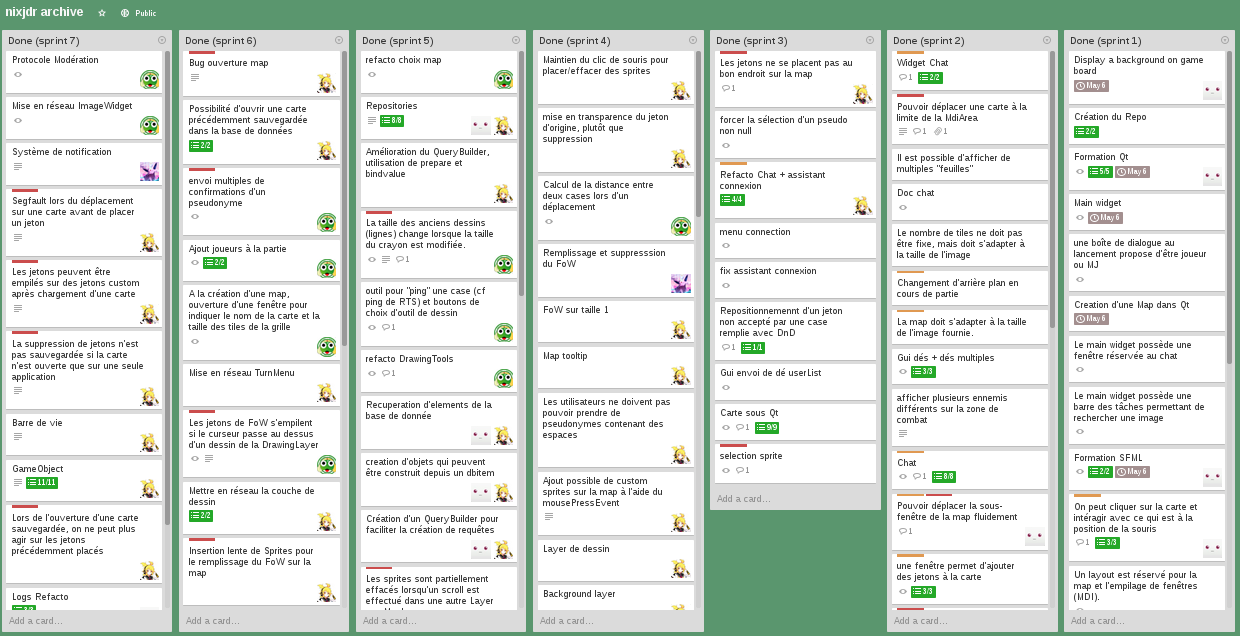
\includegraphics[width=\textwidth]{img/trello_archive.png}
	\caption{Archive de notre tableau sur Trello}
	\label{fig:trello}
\end{figure}
